\documentclass[aps,prl,twocolumn,superscriptaddress]{revtex4-1}

% the percent sign gives comments in Latex
% top line indicates this is for Physical Review, standard journal format,
% suitable for electronic submission of articles

% the line above is necessary to start any latex document.
% this is one variation that should work for most things.
% if you want double spaceing, use the following:
%
%\documentclass[prd,preprint,letterpaper]{revtex4}
%
% the "preprint" designation will make a wider line
% spacing, good for markup.
\usepackage{graphicx}  % this is the up-to-date package for all figures
\usepackage{amssymb}   % for math
\usepackage{verbatim}  % for the comment environment
\usepackage{color}
\usepackage{gensymb}
\usepackage{amsmath}

\usepackage{wrapfig}
\usepackage{hyperref}
\usepackage{titlesec}
\usepackage{amssymb}   % for math
\usepackage{verbatim}  % for the comment environment
\usepackage{color}
\usepackage[nodisplayskipstretch]{setspace}
\usepackage{amsmath}
\usepackage{blindtext}
%\usepackage[pdftex]{graphicx}
\usepackage[outdir=./]{epstopdf}
\usepackage[space]{grffile}
\usepackage{epsfig}
\usepackage[separate-uncertainty=true]{siunitx}
\usepackage{tikz}
\usepackage{pgfgantt}
\usepackage[english]{babel}
\usepackage[utf8]{inputenc}

\titlespacing*{\section}
{0pt}{1\baselineskip}{.5\baselineskip}

\titlespacing*{\subsection}
{0pt}{.5\baselineskip}{.3\baselineskip}



\bibliographystyle{apsrev}


% these are some custom control of the page size and margins
% \topmargin= 0.2in  % these 1st two may be needed for some computers
% \textheight=8.75in
%\textwidth=6.5in
%\oddsidemargin=0cm
%\evensidemargin=0cm

% this is where the actual document itself (rather than control statements) begins:

\begin{document}

% use a style that gives automatic headings
%\pagestyle{headings}



% the \title{} command generates a title.

% the \\ below is used to FORCE a line break in the middle of the sentence--
% otherwise latex computes it for you

\title{Gamma Angular Correlation in Positronium}


\author{\textbf{Bryan Yamashiro}}
\author{Christina Nelson}
\author{Corey Mutnik}
\author{Daichi Hiramatsu}
\email{byama777@hawaii.edu}
\affiliation{Department of Physics \& Astronomy, \\
University of Hawaii at Manoa,\\
2505 Correa Rd, Honolulu, HI, 96822, USA}
\altaffiliation{Quantum Lab 480L}



	      % \section is used to start a new one with a heading
\begin{abstract}

The purpose of this study is to measure fast electronics using angular correlations of the radioactive element isotopes Na$^{22}$ and Co$^{60}$.  The annihilation of Na$^{22}$ and the nuclear decay of Co$^{60}$ creates gamma ray emissions, which are detected by two organic scintillators at defined angles between 90\degree and 270\degree. Both isotope sources showed the largest rate of coincidences when the two counters were back to back. Counts were far lower at angles further away from 180\degree and showed a distribution decrease with a peak at 180\degree.





\end{abstract}

\maketitle    % this line is necessary to tell latex you are done with all
	      % of the stuff associated with the title, and now it can go
              % ahead and generate the title portion


\section{Background}


Positron Emission Tomography\,(PET) is a method of studying how organs and tissues are working using positronium annihilation\,\cite{1}. Rather than X-rays or magnetic fields, PET scans rely on use of positron isotope injection into the body. The benefits of PET scans are the ability to pick up very small areas of activity, and differentiating scar tissue\,\cite{2}. 

 % the ~\cite{ } is how you link a reference in the text. The references
 % themselves are at the end.

% one or more lines of space between paragraphs determines them

\section{Apparatus}

The apparatus includes two detectors equipped with plastic scintillators and NaI(T1) seen in figure 7. The detectors are placed at two ends with a swivel with an adjustable angle. One detector remained stationary (static) while the other detector (dynamic) angle was changed in 5\degree\,-10\degree\ increments. This angle is manipulated throughout the study to measure the angular correlation of two resultant photons. The radioactive source is placed between the two detectors and remains for the full data collection duration. Instruments used to collect data include a scaler, delay box, discriminator, and coincidence unit. The fast electronic system is shown in figure 6, and portrays the two detectors leading to the scaler that counts photon coincidences.


\section{Procedure}


\begin{table}[htb!] 
\caption{\it Initial Apparatus Parameters}
		%table caption at the top is standard
\label{t1}   % labels are used to refer to this in the text
 \begin{center}   % center the table on the page
    \begin{tabular}{|c|c|c|c|c|} \hline   % tabular environment determines the

Radioactive & Separation & Static & Dynamic & Time \\
Isotope & Distance & Voltage & Voltage & Interval  \\
  & (cm)  & (V)  & (V)  & (sec.)   \\ \hline \hline \hline
    % the "~" character forces a non-breaking space--here is just makes the columns a bit wider
Na$^{22}$ & 4 & 1500 & 1580 & 400 \\ \hline
Na$^{22}$ & 10 & 1500 & 1580  &  400  \\ \hline
Na$^{22}$ & 15 & 1500 & 1580  &  400  \\ \hline \hline
Co$^{60}$ & 4 & 1510 & 1500 &  400  \\ \hline   

     \end{tabular}
  \end{center}
\end{table}

% you always need to end an environment { } you have started--just like in C

For the Na$^{22}$ source, the collected angles included a range from 90\degree\ to 270\degree. Conversely, the Co$^{60}$ source required a range from 90\degree\ to 180\degree. The angles around 180\degree were counted in increments of 5\degree, but 10\degree elsewhere. Initial parameters for detection are included in table 1. Gamma ray emissions for the two element isotopes are generated in unique situations. Na$^{22}$ emits a pair of gamma rays by the annihilation of positronium directly opposite directions at 180\degree. Unlike this mechanism, Co$^{60}$ emits a pair of gamma rays via nuclear decay by beta decay to Ni$^{60}$\,\cite{3}.
\begin{equation}
Rate_{accidental} = R_1R_2 \Delta t
\end{equation}
The rate of accidentals is included in equation 1. The rate of accidentals were not subtracted in this study. Accidentals were muted with setup procedures by limiting the amount of double pulsing, and stacking pulse signatures in time one after the other.



\section{Calculation of Results and Errors}
% Figure placement is done automatically by Latex, but you can have some
% control: the [htb!] tells latex to try hard to place the figure 
% first here (h) then at the top (t) then the bottom (b) and the ! tells
% it to override normal concerns. Latex will still not override some
% hard rules, but this usually works. You can also move the figure around in
% the source text to help latex try to place it earlier.

Results show a Gaussian trend from the Na$^{22}$ isotope at all separation distances, portraying a count peak at 180\degree and diminishing from there. Co$^{60}$ also decreases at angles less than 180\degree. Moving the detectors further away from the source proved that counts decrease as separation distance increases. Figure 5 represents the theoretical overlapped area of the FWHM values for the three separation distances of the given initial parameters.

\subsection{Na$^{22}$ Isotope Results}




Figures 1, 2, and 3 show the angular correlation of Na$^{22}$ for three varying separation distances of the detector to the source. The 4\,cm separation had a mean of 190.17 counts with a $\sigma$ of 12.88$\pm$0.41. The 10\,cm separation had 180.14 with a $\sigma$ of 6.53$\pm$0.29. Finally, the 15\,cm separation had 176.43 counts, with a $\sigma$ of 4.30$\pm$0.19. Mean values were calculated using a least squares fit on the Gaussian fit. Three full width half maximum (FWHM) values for the corresponding separation distances were derived from the count rates along with the angles. The FWHM calculated using the normalized background as the Gaussian fit flattened were 45.23\degree\,(4\,cm), 17.03\degree\,(10\,cm), and 10.11\degree\,(15\,cm). 

\subsection{Co$^{60}$ Isotope Results}



Again using a least squares fit on figure 4, the coefficients consisted of, a$_1$\,=\,0.09\degree$\pm$0.097\degree and a$_2$\,=\,-0.04\degree$\pm$0.10\degree. Despite slight deviations, the results are consistent with theoretical expectations given the low statistics. 


\section{Discussion}


\subsection{Na$^{22}$ Isotope}
Comparing to the theoretical value of the FWHM of 47.52\degree in configuration with 4\,$\sigma$ separation, the $\sigma$ was 17.81$\pm$0.52. For 10\,cm and 15\,cm, the were 7.25$\pm$0.26 and 4.30$\pm$0.19 respectively. Figures 1, 2, and 3 show the measured element sources, but the location of the peaks are slightly off of 180\degree\, most likely from misalignment of the apparatus. In addition, the background counts are above zero. The major cause is due to the additional annihilation photon emitted from the source in coincidence with a 1.275\,MeV gamma ray. A minor factor of fluctuation is attributed to Possion fluctuation, as all counting angles were never zero.

\subsection{Co$^{60}$ Isotope}

Fits to the Co$^{60}$ data gave coefficients of a$_1$\,=\,0.09$\pm$0.097 and a$_2$\,=\,-0.04$\pm$0.10. These two values were within $\pm$1\,$\sigma$ of the theoretical expectations a$_1$\,=\,0.125 and a$_2$\,=\,0.042\,\cite{3}. The study intended to use lead shields to isolate the radioactive source, but seemed to add a significant amount of background. The background was attributed to the Compton Scattering as the detectors were not completely enclosed by the lead shields, and the shields may have added additional reflections due to the separation distance versus the decay time. The separation distance was reduced to 4\,cm, providing time for scattered rays to hit the two detectors, ultimately resulting in copious detection rates.


% the following \setlength is to force the bibliography to have no
% paragraph indentations.Can use vairous units--cm are used here.
\setlength{\parindent}{0cm}

\begin{thebibliography}{99}  % the trailing 99 controls some obscure format--just use

\bibitem{1} "PET Scan: MedlinePlus Medical Encyclopedia." U.S National Library of Medicine. U.S. National Library of Medicine. Web. 12 Oct. 2015. \url{<https://www.nlm.nih.gov/medlineplus/ency/article/003827.htm>}.     % {\em } for emphasis, \textbf{ } for boldface

\bibitem{2} Dolson, Laura. "CATs, PETs and MRIs - Getting to Know Your Scans." CATs, PETs and MRIs - Getting to Know Your Scans. Web. 12 Oct. 2015. \url{<http://www.baymoon.com/~gyncancer/library/weekly/aa071601a.htm>}.

\bibitem{3} Melissinos, A., \& Napolitano, J. (2003). Experiments in Modern Physics, Second Edition (2nd Edition ed.). New York: Academic Press.

\bibitem{4} Fast Electronics. (n.d.). Retrieved October 26, 2015, from \url{http://www.phys.hawaii.edu/~teb/fast_electronics_fernow.pdf}


\end{thebibliography}

\clearpage
\section{Figure Page}
\begin{figure}[h!]
  \begin{center}
\centerline{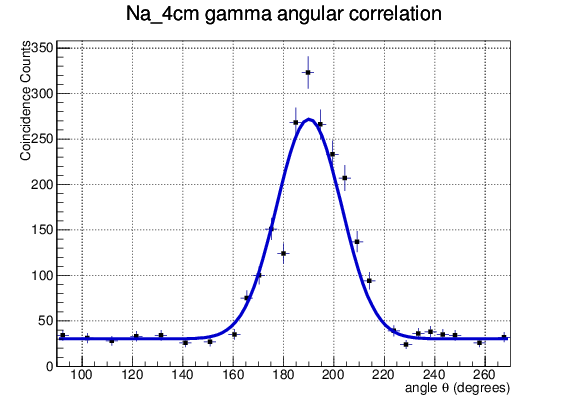
\includegraphics[width=3.in]{Na04.png}}
\caption{\it \small{Angular correlation of two photons from Na$^{22}$ at 4\,cm separation. \label{fig1}}}
  \end{center}
\end{figure}

\begin{figure}[h!]
  \begin{center}
\centerline{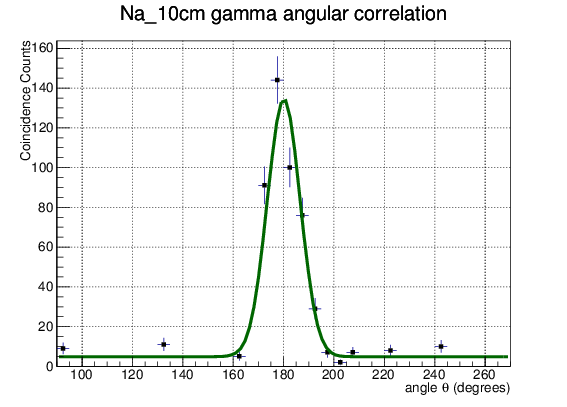
\includegraphics[width=3.in]{Na10.png}}
\caption{\it \small{Angular correlation of Na$^{22}$ at 10\,cm separation. \label{fig1}}}
  \end{center}
\end{figure}

\begin{figure}[h!]
  \begin{center}
\centerline{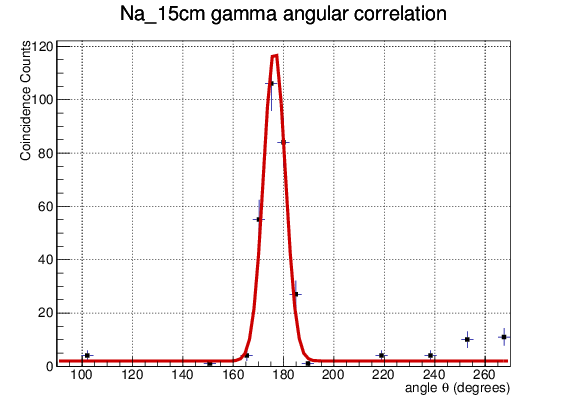
\includegraphics[width=3.in]{Na15.png}}
\caption{\it \small{Angular correlation of Na$^{22}$ at 15\,cm separation. \label{fig1}}}
  \end{center}
\end{figure}

\begin{figure}[h!]
  \begin{center}
\centerline{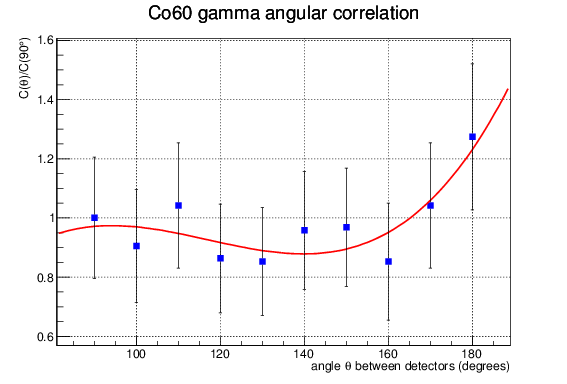
\includegraphics[width=3.in]{Co60.png}}
\caption{\it \small{Angular correlation of the $\gamma$-$\gamma$ pairs from Co$^{60}$. \label{fig1}}}
  \end{center}
\end{figure}


\begin{figure}[h!]
  \begin{center}
\centerline{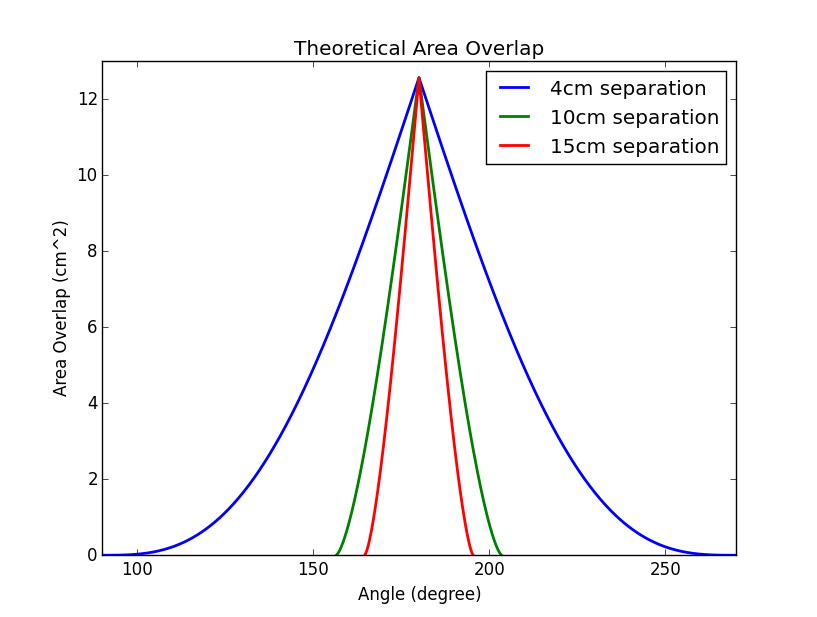
\includegraphics[width=3.in]{area.png}}
\caption{\it \small{A theoretical area overlap for the full width half maximum values for all three separation distances. \label{fig1}}}
  \end{center}
\end{figure}

\begin{figure}[h!]
  \begin{center}
\centerline{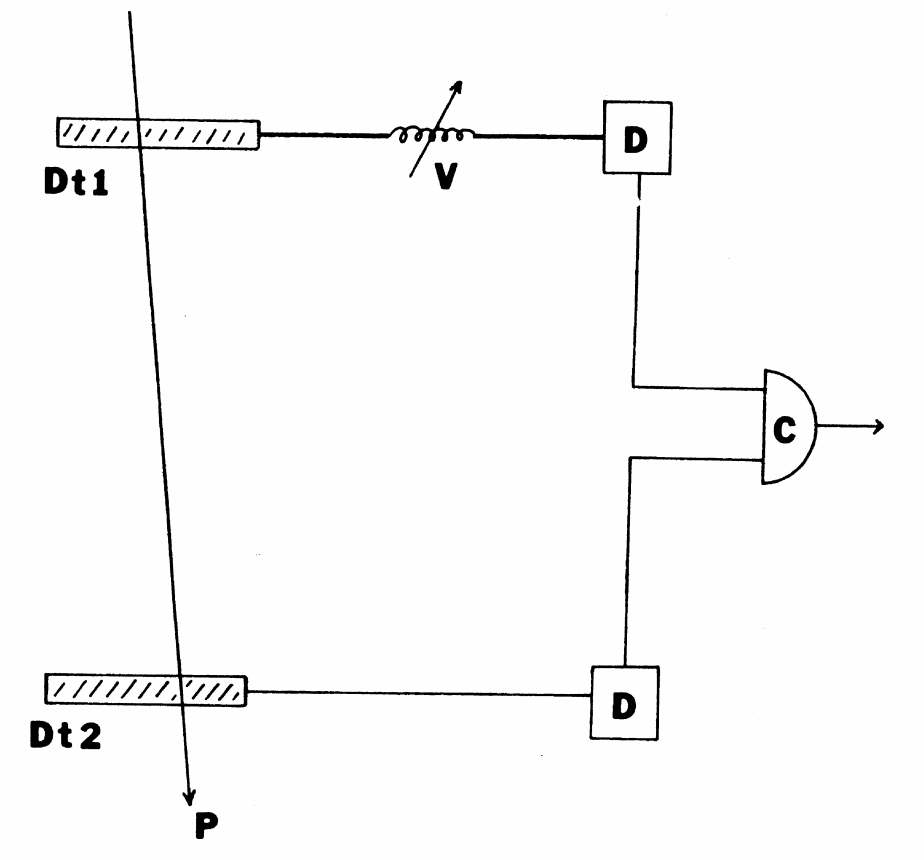
\includegraphics[width=3.in]{count.png}}
\caption{\it \small{The logic of the detector system. The photons are detected by the detectors\,(Dt1,Dt2), the signal is sent to the discriminators\,(D), and are then counted by the scaler\,(C)\,\cite{4}. \label{fig1}}}
  \end{center}
\end{figure}

\begin{figure}[h!]
  \begin{center}
\centerline{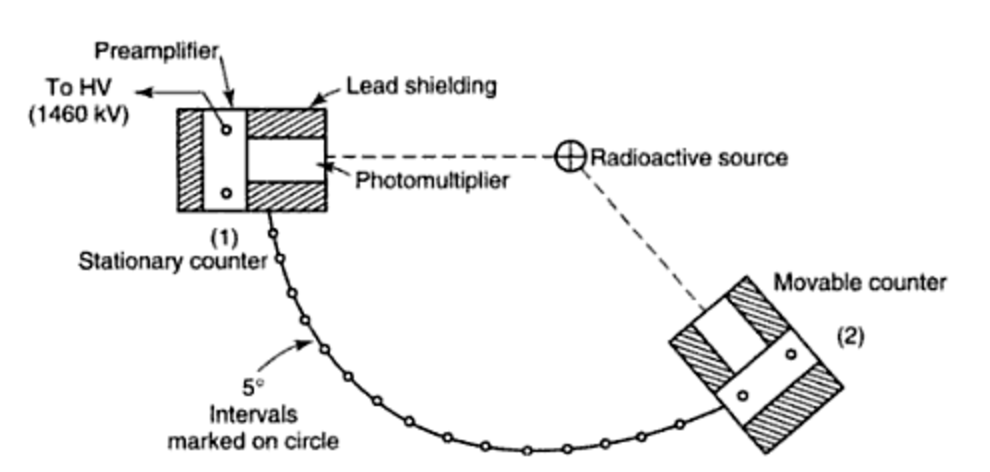
\includegraphics[width=3.in]{appar.png}}
\caption{\it \small{The detector apparatus including the two organic scintillator detectors. The angle is adjustable and was changed by a set amount of degrees to show angular correlations.\,\cite{3}. \label{fig1}}}
  \end{center}
\end{figure}


\end{document}

